
\documentclass[conference]{IEEEtran}
\usepackage[utf8]{inputenc}
\usepackage[T1]{fontenc}
\usepackage[shorthands=off,turkish]{babel}
\usepackage{cite}
\usepackage{amsmath,amssymb,amsfonts}
\usepackage{algorithmic}
\usepackage{algorithm}
\usepackage{graphicx}
\usepackage{textcomp}
\usepackage{xcolor}
\usepackage{booktabs}
\usepackage{multirow}
\usepackage{array}
\usepackage{url}

\begin{document}

\title{Destek Sınırlı Klinik Koşullar Altında Sepsis Dozaj Politikaları İçin Orkestre Edilmiş Bir Çevrimdışı Pekiştirmeli Öğrenme İş Akışı}

\author{
\IEEEauthorblockN{Furkan Nezih Üzmez}
\IEEEauthorblockA{230202073}
}

\maketitle

\begin{abstract}
Bu rapor, MIMIC-IV tabanlı sepsis kohortunda intravenöz sıvı ve vazopresör tedavi kararlarını değerlendirmek için geliştirilen uçtan uca, zero-leakage ve yeniden üretilebilir bir offline pekiştirmeli öğrenme iş akışını sunar. Çalışma canlı hastalar üzerinde çevrimiçi keşif yapmaz; yalnızca retrospektif yoğun bakım kayıtlarından model-free, off-policy ve offline politika öğrenimi yapar. Proje Sepsis-3 kohort seçimi, 72 saatlik klinik pencereleme, 62 boyutlu durum temsili, $5\times5$ ayrık aksiyon uzayı, sparse ve SOFA-shaped ödül varyantları, train-only preprocessing, hasta-düzeyi split, IQL hiperparametre taraması, çok kriterli finalist seçimi, çoklu tohum doğrulaması, off-policy evaluation ve raporlanabilir grafik artifactlerini kapsar. Final IQL taraması iki ödül varyantı, üç learning-rate rejimi ve üç expectile-temperature ayarından oluşan on sekiz konfigürasyonu Aşama 1'de değerlendirir; Aşama 2'de seçilen altı finalist üç tohumla doğrulanır. Güncel sonuçlar, final seçili politikanın SOFA-shaped ödül, konservatif learning-rate ve safe IQL ayarını kullanan `iql\_sofa\_shaped\_conservative\_safe' konfigürasyonu olduğunu gösterir. Bu aday üç tohum ortalamasında FQE=2.848, WIS=8.203, bootstrap WIS 95\% CI=4.963--10.817, ESS=29.410, destek kütlesi=0.991 ve klinisyen exact-bin uyumu=0.414 elde etmiştir. ESS 50 eşiğinin altında kaldığından sonuç klinik üstünlük kanıtı olarak değil, destek kısıtı açıkça raporlanan retrospektif off-policy değerlendirme kanıtı olarak yorumlanmalıdır.
\end{abstract}

\begin{IEEEkeywords}
offline pekiştirmeli öğrenme, implicit Q-learning, sepsis, MIMIC-IV, off-policy evaluation, yeniden üretilebilirlik, klinik karar desteği
\end{IEEEkeywords}

\section{Giriş}
Sepsis tedavisi, belirsizlik altında ardışık kararlar, gecikmeli sonuçlar ve klinik şiddete bağlı confounding içeren bir yoğun bakım problemidir. Offline pekiştirmeli öğrenme, hasta üzerinde yeni denemeler yapmadan tarihsel klinik trajektorilerden politika öğrenmeyi sağlar. Bu özellik tıbbi ortamda kritiktir; çünkü çevrimiçi keşif etik olarak kabul edilemez. Ancak offline öğrenme, desteklenmeyen aksiyonlara kayma, yüksek varyanslı off-policy estimatorler ve validasyon artifactlerine aşırı uyum gibi riskler taşır.

Bu projenin amacı, MIMIC-IV verisi üzerinde sepsis tedavisi için güvenilir bir klinik karar destek değerlendirme altyapısı kurmaktır. Sistem yatak başı canlı tedavi aracı değildir; geriye dönük offline policy evaluation ve model karşılaştırma laboratuvarıdır. Model sınıfı model-free, off-policy ve offline RL'dir; proje genelinde CQL, BCQ ve IQL aileleri değerlendirme bağlamında düşünülmüş, final rapor odağı IQL olarak belirlenmiştir. Kod tabanı cihaz-bağımsız çalışacak şekilde tasarlanmıştır; Apple Silicon MPS ve NVIDIA CUDA ortamlarında aynı eğitim mantığıyla çalışması hedeflenmiştir.

Bu proje, MIMIC-IV tabanlı sepsis kohortunda dört saatlik karar pencereleriyle retrospektif politika değerlendirmesi yapar. Aksiyon uzayı, vazopresör ve intravenöz sıvı şiddetinin $5\times5$ ayrık kombinasyonudur. Final deneyin amacı IQL konfigürasyonlarını iki ödül varyantı altında karşılaştırmak, güvenilir finalistleri yalnız validasyon kanıtıyla seçmek ve raporlanabilir bir artifact bundle üretmektir. Bu çalışmada protokol, açık denetim kapıları, deterministik konfigürasyon genişletmesi, çoklu tohum birleştirmesi ve grafik raporlama ile çalışır hale getirilmiştir.

\section{İlgili Çalışmalar}
Offline pekiştirmeli öğrenme sabit veri kümelerinden politika öğrenme problemine odaklanır. IQL, veri dışı aksiyonları doğrudan maksimize etmek yerine expectile value learning ve advantage-weighted behavioral cloning kullanarak konservatif offline ortamlara uygun bir yaklaşım sunar \cite{iql}. Bu tercih CQL gibi açık Q-cezası kullanan yöntemlere göre daha sade bir seçimdir: CQL extrapolation error riskini doğrudan cezalandırır, fakat ceza ağırlığı yanlış seçildiğinde klinik olarak makul ama nadir aksiyonları aşırı bastırabilir \cite{cql}. IQL ise veri içi Q yedekleriyle ve davranış klonlamasına yakın politika çıkarımıyla destek dışına taşmayı azaltır; bunun bedeli, veri dağılımında hiç temsil edilmeyen tedavi stratejilerini keşfedememesidir.

Sepsis alanında RL çalışmalarının temel örnekleri, sıvı ve vazopresör dozlarını ayrık tedavi aksiyonları olarak modelleyen AI Clinician çalışması ve sürekli durum temsiliyle optimal sepsis tedavisi öğrenmeye çalışan derin RL yaklaşımıdır \cite{komorowski2018ai,raghu2017sepsis}. Bu çizgideki sonuçlar klinik karar desteği için umut verici olsa da, sağlıkta RL rehberleri gözlemsel veriden öğrenilen politikaların confounding, destek eksikliği, estimator varyansı ve prospektif doğrulama eksikliği nedeniyle doğrudan tedavi önerisi sayılamayacağını vurgular \cite{gottesman2019guidelines}. Bu nedenle bu raporun amacı da klinik üstünlük iddiası üretmek değil, raporlanabilir ve yeniden üretilebilir bir offline değerlendirme kanıtı oluşturmaktır. Veri temeli, de-identified kritik bakım kayıtları sağlayan MIMIC-IV veri tabanıdır \cite{mimiciv}; tedavi aksiyonlarının sıvı ve vazopresör eksenlerinde kurulması ise sepsis ve septik şok yönetiminde bu iki müdahalenin merkezi rol oynadığı güncel kılavuzlarla uyumludur \cite{evans2021ssc}.

\section{Kuramsal Arka Plan ve Algoritmik Konumlandırma}
Offline RL'de temel gerilim, politika iyileştirmesi ile veri desteği dışına taşmama zorunluluğu arasındadır. Klasik off-policy değer öğrenimi, bir sonraki durumda $\max_{a'} Q(s',a')$ gibi veri setinde gözlenmemiş aksiyonları sorguladığında, fonksiyon yaklaştırıcıların eğitim sinyali almadığı bölgelerde extrapolation error oluşur. Bu hata Bellman yedeklemeleriyle tekrar tekrar taşınır ve özellikle klinik veri gibi seyrek, heterojen ve confounded alanlarda politikayı güvenilmez doz önerilerine yöneltebilir.

Bu riske karşı literatürde üç ana yaklaşım öne çıkar. Birincisi, CQL gibi explicit action-space regularization yöntemleridir; bu yöntemler veri dışı aksiyonların Q değerlerini cezalandırarak kötümser bir alt sınır kurar \cite{cql}. İkincisi, IQL gibi implicit ve in-sample regularization yöntemleridir; bu yöntemler gözlenmemiş aksiyonları doğrudan sorgulamak yerine veri içi aksiyonların üst expectile değerlerini öğrenir \cite{iql}. Üçüncüsü, daha yeni state-space manifold regularization fikirleridir; bunlar aksiyon uzayı yerine durum manifoldunun dışındaki bölgelerde value fonksiyonunu cezalandırmayı önerir. Bu proje klinik güvenlik ve uygulama sadeliği nedeniyle IQL hattını kullanır, fakat CQL ve state-space regularization fikirlerini sonuçların yorumlanmasında karşılaştırmalı arka plan olarak dikkate alır.

Referans araştırma taslaklarında vurgulanan multi-step value propagation fikri de bu çalışma için önemli bir gelecek yönüdür. Tek adımlı yedeklemeler sparse terminal mortalite sinyalini uzun trajectory boyunca yavaş taşır; Peng'in $Q(\lambda)$ gibi eligibility trace tabanlı yaklaşımlar bu sinyali daha hızlı yayabilir. Ancak mevcut klinik final raporda, önce destek güvenliği ve leakage-free değerlendirme sabitlenmiş; multi-step operatörler daha sonra eklenecek araştırma ekseni olarak bırakılmıştır. Bu tercih yapılmasaydı final IQL sonucunun etkisi, aynı anda değişen yedekleme operatörü ve güvenlik protokolü nedeniyle ayrıştırılamazdı.

\section{Uçtan Uca Proje Mimarisi}
Proje, katı bağımlılık zinciriyle ilerleyen on ana adımdan oluşur. Bu yapı, veri hazırlama hatalarının final politika değerlendirmesine taşınmasını engellemek için bilinçli olarak aşamalı tasarlanmıştır.

\begin{table*}[t]
\centering
\caption{Projenin on aşamalı uçtan uca mimarisi.}
\label{tab:ten_steps}
\begin{tabular}{p{0.08\textwidth}p{0.25\textwidth}p{0.58\textwidth}}
\toprule
Adım & Bileşen & İçerik \\
\midrule
1 & Kohort seçimi & MIMIC-IV içinden Sepsis-3 kriterlerine uyan yetişkin ICU hastalarının seçilmesi; geçersiz onset, kısa ICU kalışı, eksik temel demografi ve tekrar yatışların yönetilmesi. \\
2 & Zaman çizelgesi & Sepsis onset'inden 24 saat önce başlayıp 48 saat sonrasına uzanan 72 saatlik pencerenin 4 saatlik karar adımlarına bölünmesi. \\
3 & Zero-leakage split & Hastaların train/validation/test olarak hasta-düzeyinde ayrılması ve preprocessing fit işlemlerinin yalnız train üzerinde yapılması. \\
4 & State çıkarımı & Vital, laboratuvar, tedavi geçmişi, demografi, missingness ve türetilmiş değişkenlerden 62 boyutlu durum vektörü üretilmesi. \\
5 & Action/reward & Vazopresör ve IV sıvı dozlarının 25 ayrık aksiyona dönüştürülmesi; sparse ve SOFA-shaped ödüllerin üretilmesi. \\
6 & Transition/baseline & Replay verisinin $(s_t,a_t,r_t,s_{t+1},done_t)$ formatında yazılması; clinician, no-treatment ve behavior cloning baselinelarının kurulması. \\
7--8 & IQL eğitimi & Offline veride destek dışına çıkmadan expectile value learning ve advantage-weighted actor update ile IQL politikalarının eğitilmesi. \\
9 & OPE ve güvenlik & FQE, WIS, ESS, bootstrap CI, destek kütlesi, clinician agreement, heatmap ve güvenlik diagnostiklerinin hesaplanması. \\
10 & Final sweep & 18 konfigürasyonlu IQL taraması, finalist seçimi, çoklu tohum doğrulaması ve IEEE rapor artifactlerinin üretilmesi. \\
\bottomrule
\end{tabular}
\end{table*}

Bu mimari tek bir eğitim scriptinden daha fazlasıdır: kohort tanımı, veri sözleşmesi, model eğitimi, off-policy değerlendirme, güvenlik analizi ve raporlama artifactleri aynı deney protokolünün parçalarıdır. Böyle seçilmeseydi final IQL sonucu üretilebilir görünse bile, veri hazırlama, split sızıntısı veya preprocessing farkı gibi alt seviye hatalar model başarısı sanılabilirdi.

\section{Kohort, Zaman ve Split Tasarımı}
\subsection{Kohort Seçimi}
Kohort MIMIC-IV üzerinde Sepsis-3 kriterlerine göre oluşturulur \cite{singer2016sepsis3,mimiciv}. Dahil edilen popülasyon 18 yaş ve üzeri yetişkin, doğrudan ICU izlemine sahip ve sepsis tanımıyla uyumlu hastalardır. Çocuk hastalar farklı doz ve fizyoloji rejimlerine sahip oldukları için dışarıda bırakılır; bu karar verilmeseydi model tek bir aksiyon-doz anlamını heterojen yaş grupları için öğrenmeye zorlanırdı. ICU dışı veya yoğun gözlem verisi olmayan hastalar da dışlanır; çünkü 4 saatlik karar pencereleri için yeterli fizyolojik zaman serisi kurulamaz.

Dışlama kuralları metodolojik güvenlik için açık tutulmuştur. Sepsis onset zamanı bulunamayan hastalar, 4 saatten kısa ICU kalışı olanlar ve yaş/cinsiyet gibi temel demografisi eksik olanlar çıkarılır. Tekrar yatan hastalarda yalnız ilk yatış kullanılır. Bu en kritik zero-leakage kararlarından biridir: aynı hastanın bir yatışı train setine, sonraki yatışı test setine düşerse model hasta anatomisini veya kronik profilini dolaylı olarak ezberleyebilir. Filtreleme sonucu ve dışlanan hasta sayıları audit artifactleriyle belgelenir.

\subsection{Zaman Çizelgesi}
Her ICU kalışı için `sepsis\_onset\_time' hesaplanır. Analiz penceresi onset'ten 24 saat önce başlayıp 48 saat sonrasına kadar devam eder. Bu 72 saatlik pencere 4 saatlik karar adımlarına ayrıldığında tipik episode yaklaşık 18 timestep içerir. Dört saatlik pencere, literatürdeki sepsis RL kurulumlarıyla karşılaştırılabilirlik sağlar ve klinik ölçümlerin düzensiz zamanlanmasını yönetilebilir bir karar frekansına indirger \cite{komorowski2018ai,raghu2017sepsis}. Daha kısa pencere seçilseydi ölçüm eksikliği ve gürültülü aksiyon tekrarları artacak, davranış politikası olasılıkları daha seyrek gözlenen mikro kararlar üzerinde tahmin edilecekti. Daha uzun pencere seçilseydi de sıvı ve vazopresör değişimlerinin akut fizyolojik etkileri ortalamaya karışacak, ardışık karar yapısı zayıflayacaktı.

\subsection{Split Stratejisi}
Varsayılan split hasta düzeyinde train \%70, validation \%15 ve test \%15 olarak yapılır. Split seed'i 42 olarak sabitlenir. Train, validation ve test subject kümelerinin kesişimi boş olmalıdır. Test seti yalnız final raporlama için kullanılır; hyperparameter, checkpoint veya metrik tasarımı test sonucuna göre değiştirilmez. Bu kural ihlal edilseydi final test metrikleri gerçek held-out kanıt olmaktan çıkar, validasyonun uzantısı haline gelirdi.

\section{MDP Formülasyonu}
Problem sonlu ufuklu bir Markov karar süreci olarak modellenir:
\begin{equation}
M=(S,A,P,R,\gamma).
\end{equation}
Burada $S$ hasta durum uzayını, $A$ ayrık tedavi aksiyonlarını, $P$ geçiş dinamiklerini, $R$ ödül fonksiyonunu ve $\gamma$ discount factor'ü temsil eder. Her geçiş şu biçimdedir:
\begin{equation}
(s_t,a_t,r_t,s_{t+1},done_t).
\end{equation}

\subsection{State Temsili}
State vektörü hastanın o andaki klinik durumunu özetleyen 62 sürekli/ikili özellikten oluşur. Başlıca gruplar kalp hızı, MAP, sistolik/diyastolik tansiyon, solunum ve SpO2 gibi vital bulgular; kan gazı, elektrolit, renal, hepatik, koagülasyon ve hemogram laboratuvarları; kümülatif sıvı, vazopresör maruziyeti ve idrar çıkışı gibi tedavi sinyalleri; yaş ve cinsiyet gibi demografik değişkenler; PaO2/FiO2, shock index ve onset sonrası saat gibi türetilmiş değişkenlerdir.

Her 4 saatlik pencerede birden fazla ölçüm varsa özelliğe göre `last', `mean', `min', `max', `sum' veya `cumulative' agregasyon kuralı uygulanır. Örneğin bazı vital bulgularda son ölçüm klinik karar anına daha yakın bilgi taşırken, toplam sıvı veya kümülatif vazopresör maruziyeti pencere içi tedavi yükünü temsil eder. Tek bir agregasyon kuralı tüm değişkenlere dayatılsaydı klinik anlamı farklı sinyaller aynı istatistiksel kalıba sıkıştırılmış olurdu.

Eksik veriler için sıralı strateji uygulanır: episode içinde forward-fill, train split üzerinden hesaplanan medyan, klinik normal değer fallback ve gerekli durumda missingness flag. Missingness göstergeleri eklenmeseydi model, ölçülmeyen laboratuvarı normal değerle karıştırabilir ve hekimin ölçüm kararıyla taşınan risk bilgisini kaybedebilirdi. Train-only medyan kullanılmasaydı validation/test dağılım bilgisi preprocessing üzerinden eğitime sızardı.

\subsection{Action Uzayı}
Aksiyon uzayı 25 ayrık tedavi kararından oluşur. Her aksiyon, vazopresör dozu ve IV sıvı miktarının $5\times5$ kombinasyonudur:
\begin{equation}
action\_id = vaso\_bin \times 5 + fluid\_bin.
\end{equation}
Bin 0 tedavi yok anlamına gelir; non-zero dozlar train split üzerindeki çeyrekliklere göre Q1--Q4 olarak ayrılır. Zero dose ayrı tutulur, çünkü hiç tedavi vermemek küçük ama non-zero tedaviyle aynı klinik anlamı taşımaz. Bin eşikleri yalnız train split üzerinde öğrenilir ve validation/test üzerinde dondurulmuş şekilde uygulanır. Eşikler tüm veri üzerinde hesaplansaydı test doz dağılımı aksiyon kodlamasına sızardı.

\begin{table}[t]
\centering
\caption{Vazopresör ve IV sıvı aksiyon grid'i.}
\label{tab:action_grid}
\begin{tabular}{c|ccccc}
\toprule
 & \multicolumn{5}{c}{Sıvı bini} \\
Vazo bini & 0 & 1 & 2 & 3 & 4 \\
\midrule
0 & 0 & 1 & 2 & 3 & 4 \\
1 & 5 & 6 & 7 & 8 & 9 \\
2 & 10 & 11 & 12 & 13 & 14 \\
3 & 15 & 16 & 17 & 18 & 19 \\
4 & 20 & 21 & 22 & 23 & 24 \\
\bottomrule
\end{tabular}
\end{table}

\subsection{Reward Tasarımı}
İki ödül varyantı kullanılır. Sparse ödül yalnız terminal mortalite/sağkalım utility'sini kullanır: 90 gün yaşayan hasta için $+15$, 90 gün içinde ölüm için $-15$. Bu seçenek klinik nihai sonucu doğrudan hedeflediği için yorumlanması kolaydır, fakat uzun ufuklu ve seyrek geri bildirimli olduğundan değer öğrenmesi yüksek varyanslı hale gelebilir.

SOFA-shaped ödül terminal utility'yi korur ve ara adımlarda SOFA değişimine küçük bir shaping sinyali ekler:
\begin{equation}
sofa\_shaping = -0.025 \times (SOFA_{current}-SOFA_{previous}).
\end{equation}
SOFA artışı kötüleşme olarak negatif, SOFA azalması iyileşme olarak pozitif sinyal üretir. SOFA'nın sepsis organ disfonksiyonu tanımı ve klinik şiddet takibiyle ilişkili olması bu ara sinyali klinik olarak gerekçelendirir \cite{singer2016sepsis3}. SOFA shaping kullanılmasaydı eğitim yalnız terminal sonuca dayanacak ve ara fizyolojik iyileşmeleri ayırt etmek zorlaşacaktı. Tersine, shaping ağırlığı çok güçlü seçilseydi ajan mortalite yerine kısa vadeli skor oynamalarını optimize edebilirdi; bu nedenle terminal utility korunmuş ve seçim ortak terminal değerlendirmeye bağlanmıştır.

\subsection{Discount Factor}
Discount factor $\gamma=0.99$ olarak sabitlenir. Bu seçim, sepsis tedavisinde kısa vadeli hemodinamik kararların uzun vadeli mortalite sonucuyla ilişkili olması nedeniyle uygundur. Daha küçük bir $\gamma$ kısa vadeli SOFA değişimlerini fazla öne çıkarabilir, $\gamma=1$ ise sonlu ufukta mümkün olsa da FQE ve WIS tahminlerinde geç dönem terminal sinyallerine daha hassas bir varyans profili doğurabilirdi.

\section{Preprocessing ve Leakage-Free Sözleşmeler}
Temel kural `fit on train, transform everywhere' şeklindedir. Scaler parametreleri, imputer medyanları, clip bound veya percentile eşikleri, action bin quartile eşikleri, behavior policy estimator, FQE estimator ve normalization sabitleri train üzerinde fit edilir. Validation ve test üzerinde yalnız train'de fit edilmiş transformlar uygulanır.

Fizyolojik olarak makul olmayan değerler valid range dışında filtrelenir veya clip edilir. Clipping ve normalization parametreleri train split üzerinde fit edilir. Bu tercih yapılmasaydı validation/test dağılımının uç değer bilgisi eğitim öncesi veri dönüşümlerine yansıyabilir ve raporlanan performans fazla iyimser olurdu.

\subsection{Aşama 0 Ön Tarama Denetimi}
Presweep denetimi, final eğitim sonucunun raporlanabilir sayılmasından önce veri sözleşmelerini kontrol eder. Bu kapı özellikle sağlıkta RL için gereklidir; çünkü küçük bir split sızıntısı veya outcome leakage, gözlemsel klinik veride gerçek politika kalitesinden çok daha büyük görünen kazançlar üretebilir \cite{gottesman2019guidelines}. Denetim şu maddeleri kapsar: sparse replay üretimi, sparse ve SOFA-shaped replay artifactlerinde aynı patient split/preprocessing/action bin/transition indexing/terminal outcome tanımlarının kullanılması, action binlerinin train-only fit edilmesi, imputation/scaling/clipping/normalization istatistiklerinin train-only olması, validation FQE'nin ortak terminal survival/death reward ile çalışması, temporal alignment kontrolü, splitler arası hasta çakışması bulunmaması ve mortality/discharge/gelecek outcome bilgisinin state feature'larına sızmaması.

\begin{table}[t]
\centering
\caption{Presweep denetim özeti.}
\label{tab:audit}
\begin{tabular}{lrrr}
\toprule
Kanıt kalemi & Train & Validation & Test \\
\midrule
Split manifest satırı & 12063 & 2585 & 2585 \\
SOFA-shaped replay satırı & 140635 & 30539 & 30046 \\
Sparse replay satırı & 140635 & 30539 & 30046 \\
\midrule
Split leakage & \multicolumn{3}{c}{Başarılı} \\
Ortak replay sözleşmesi & \multicolumn{3}{c}{Başarılı} \\
Zamansal hizalama & \multicolumn{3}{c}{Başarılı} \\
Outcome leakage taraması & \multicolumn{3}{c}{Başarılı} \\
\bottomrule
\end{tabular}
\end{table}

Bu adım atlanmış olsaydı Aşama 2 sonucu sayısal olarak üretilebilir görünse bile, aynı hastanın farklı splitlere düşmesi veya terminal bilginin özelliklere sızması nedeniyle metodolojik olarak geçersiz hale gelebilirdi.

\section{Baseline Politikaları}
Final test karşılaştırması üç referans politika içerir. Clinician replay, replay datasetindeki gözlenen klinisyen aksiyonlarını değerlendirir ve davranış verisinin kendisini referans alır. No-treatment policy, uygun yerlerde no-vasopressor/no-fluid bin'ini seçen basit kontrol politikasıdır. Behavior cloning ise klinisyen aksiyonlarını supervised learning ile taklit eder. Bu baselinelar eklenmeseydi IQL çıktısı yalnız kendi OPE skoru ile raporlanır, davranış politikasına ve basit kontrol stratejilerine göre bağlamı kaybolurdu.

\section{IQL Algoritması}
Implicit Q-Learning, offline RL için geliştirilmiş ve dataset dışındaki aksiyonları doğrudan maksimize ederek extrapolation error üretmekten kaçınan bir algoritmadır \cite{iql}. IQL üç bileşen kullanır: critic, value function ve actor. Critic $Q_\theta(s,a)$ state-action değerini tahmin eder. Value function klasik max operator yerine expectile regression ile öğrenilir. Expectile parametresi value hedefinin Q dağılımının hangi bölgesine yaklaşacağını belirler; daha düşük expectile daha konservatif, daha yüksek expectile daha optimistic value tahmini üretir.

Value objective asimetrik expectile kaybı ile yazılır:
\begin{equation}
L_V(\psi)=\mathbb{E}_{(s,a)\sim D}\left[L_2^\tau(Q_\theta(s,a)-V_\psi(s))\right],
\end{equation}
\begin{equation}
L_2^\tau(u)=|\tau-\mathbb{I}(u<0)|u^2.
\end{equation}
$\tau$ 1'e yaklaştıkça value fonksiyonu davranış verisi içinde daha iyi görünen aksiyonların üst expectile'ına yaklaşır. Q fonksiyonu ise veri dışı aksiyon maksimumu yerine öğrenilen state value hedefiyle güncellenir:
\begin{equation}
L_Q(\theta)=\mathbb{E}_{D}\left[(r+\gamma V_\psi(s')-Q_\theta(s,a))^2\right].
\end{equation}

Actor, dataset içindeki aksiyonları advantage'a göre ağırlıklandırarak öğrenir:
\begin{equation}
A(s,a)=Q_\theta(s,a)-V_\psi(s),
\end{equation}
\begin{equation}
L_\pi(\phi)=\mathbb{E}_{D}\left[\exp(\beta A(s,a))\log \pi_\phi(a|s)\right].
\end{equation}
Burada $\beta$ ya da temperature politika çıkarımının agresifliğini kontrol eder. Düşük temperature davranış politikasına daha yakın ve konservatif politika çıkarır; yüksek temperature potansiyel getiriyi artırabilir fakat düşük destekli aksiyonlara kayma riskini de büyütür. Bu nedenle safe, baseline ve optimistic ayarları birlikte denenmiştir.

\section{IQL Final Tarama Tasarımı}
Final tarama iki ödül varyantı, üç learning-rate rejimi ve üç IQL ayarını on sekiz Aşama 1 adayına genişletir. Learning-rate rejimleri actor, critic ve value optimizasyonunu ayrı olarak kontrol eder. Konservatif learning-rate rejimi finalde öne çıkarılmıştır; çünkü offline RL'de agresif critic güncellemeleri veri dışı Q tahminlerini büyütebilir ve politika çıkarımı bu hataları çoğaltabilir \cite{cql,iql}. Baseline rejim yalnızca referans anchor olarak tutulmuştur; hiç denenmeseydi konservatif seçimin gerçekten gerekli olup olmadığı gözlenemezdi. Actor-konservatif rejim ise politika güncellemelerini yavaşlatmanın, critic/value öğrenmesini tamamen yavaşlatmadan destek uyumunu artırıp artırmadığını test eder.

\begin{table*}[t]
\centering
\caption{Final IQL hiperparametre grid'i.}
\label{tab:grid_full}
\begin{tabular}{lll}
\toprule
Boyut & Seçenek & Değerler \\
\midrule
Reward & sparse & terminal survival/death utility \\
Reward & SOFA-shaped & terminal utility + SOFA değişim shaping \\
LR rejimi & conservative & actor $3\times10^{-5}$, critic $1\times10^{-4}$, value $1\times10^{-4}$ \\
LR rejimi & baseline & actor $1\times10^{-4}$, critic $3\times10^{-4}$, value $3\times10^{-4}$ \\
LR rejimi & actor-conservative & actor $3\times10^{-5}$, critic $3\times10^{-4}$, value $3\times10^{-4}$ \\
IQL ayarı & safe & expectile 0.7, temperature 1.0 \\
IQL ayarı & baseline & expectile 0.7, temperature 3.0 \\
IQL ayarı & optimistic & expectile 0.8, temperature 3.0 \\
\bottomrule
\end{tabular}
\end{table*}

\begin{table}[t]
\centering
\caption{Sabit eğitim parametreleri.}
\label{tab:fixed_params}
\begin{tabular}{ll}
\toprule
Parametre & Değer \\
\midrule
Algoritma & IQL \\
Epoch & 200 \\
Batch size & 256 \\
Discount & 0.99 \\
Policy hidden sizes & [256, 256] \\
Value hidden sizes & [256, 256] \\
Critic hidden sizes & [256, 256] \\
Polyak tau & 0.005 \\
Target update freq & 10 \\
Grad clip & 10.0 \\
Device & auto \\
\bottomrule
\end{tabular}
\end{table}

Sabit parametreler korunmuştur; böylece final sweep yalnız reward, learning-rate rejimi, expectile ve temperature etkisini ölçer. Bu parametreler de serbest bırakılsaydı 18 konfigürasyonun etkisi yorumlanamaz, model başarısının mimari mi yoksa reward/LR/IQL ayarı kaynaklı mı olduğu belirsizleşirdi.

\begin{algorithm}[t]
\caption{Final IQL Tarama ve Raporlama İş Akışı}
\label{alg:workflow}
\begin{algorithmic}[1]
\STATE Replay, split, preprocessing ve zamansal sözleşmeleri doğrula
\STATE Ödül, learning-rate ve IQL ayarlarını genişlet
\FOR{her Aşama 1 adayı}
  \STATE Seed 42 ile politikayı eğit
  \STATE Validasyon metriklerini ve destek diagnostiklerini hesapla
\ENDFOR
\STATE Güvenlik veya destek kapılarını geçemeyen adayları işaretle
\STATE Composite, ödül dengesi, güvenlik ve çeşitlilik slotlarıyla finalist seç
\FOR{her finalist ve her doğrulama tohumu}
  \STATE Seed 123 ve 456 ile politikayı eğit veya yeniden kullan
  \STATE Çoklu tohum değerlendirme kanıtını topla
\ENDFOR
\STATE Tekrarlanan tohum kanıtıyla final konfigürasyonu seç
\STATE Baseline karşılaştırmaları, grafikler ve yeniden üretilebilirlik artifactleri üret
\end{algorithmic}
\end{algorithm}

\section{Seed Stratejisi ve Karar Kuralı}
Final rapor için tek seed yeterli değildir. Offline RL eğitiminde initialization, minibatch sırası ve stochastic optimizasyon sonucu etkileyebilir. Aşama 1'de 18 konfigürasyon seed 42 ile taranır. Hesaplama verimli olsun diye tüm $2\times3\times3\times3=54$ run doğrudan çalıştırılmamış, önce tek seed tarama yapılmış, ardından umut vadeden finalistler ek seedlerle doğrulanmıştır. Compute kısıtlı durumda önerilen tasarım 18 + (6 x 2) = 30 run'dır. Bu tasarım 54 run'lık tam grid'e göre daha ekonomiktir; yine de finalist konfigürasyonlar üç seed ile doğrulandığı için final raporda seed varyansı ve stabilite analizi raporlanabilir.

Hyperparameter seçimi test set üzerinden yapılmaz. Seçim validation split üzerindeki FQE, WIS, ESS, clinician agreement, action distribution makullüğü, low-support action uyarıları, reward curve ve training stability sinyallerine dayanır. Tek bir metrikle karar verilmez. Örneğin yüksek WIS ama çok düşük ESS varsa bu sonuç güvenilir kabul edilmez.

Bir konfigürasyon final aday olmadan önce validation performansı rekabetçi olmalı, ESS çok düşük olmamalı, FQE sonucu WIS ile tamamen çelişmemeli, action distribution klinik olarak makul olmalı, low-support action oranı kabul edilebilir düzeyde olmalı, farklı seedlerde performans tamamen kararsız olmamalı ve test set seçim sürecinde kullanılmamış olmalıdır.

\section{Aşama 1 Finalist Seçim Sonuçları}
Aşama 1 seçici altı finalist üretmiştir. En yüksek iki aday SOFA-shaped ödül ve konservatif learning-rate kullanırken, diğer slotlar sparse ödül temsilini, güvenlik-destek dengesini, baseline anchor seçimini ve çeşitlilik backfill kuralını korur. Tablo~\ref{tab:finalists}, seçilen adayları ve ana validasyon diagnostiklerini gösterir.

\begin{table*}[t]
\centering
\caption{Aşama 1 final-altı seçim özeti.}
\label{tab:finalists}
\begin{tabular}{rllllrrrr}
\toprule
Sıra & Slot & Ödül & LR & IQL & FQE & WIS & Destek & Uyum \\
\midrule
1 & top composite & SOFA & konservatif & safe & 3.169 & 8.616 & 0.965 & 0.418 \\
2 & top composite & SOFA & konservatif & baseline & 2.280 & 7.009 & 0.973 & 0.401 \\
3 & best sparse & sparse & konservatif & safe & 1.954 & 8.740 & 0.971 & 0.411 \\
4 & safety support & sparse & baseline & baseline & 1.421 & 6.768 & 0.973 & 0.410 \\
5 & baseline anchor & sparse & baseline & safe & 2.345 & 8.125 & 0.963 & 0.416 \\
6 & diversity backfill & sparse & konservatif & baseline & 2.012 & 7.782 & 0.969 & 0.407 \\
\bottomrule
\end{tabular}
\end{table*}

Seçilen küme, protokolün tek skorlu sıralama yerine çok kriterli ve çeşitlilik koruyan seçim hedefiyle uyumludur. Klinik offline öğrenmede bu önemlidir; çünkü yüksek value tahmini, zayıf davranış desteği veya aşırı dağılım kayması durumunda güvenilir olmayabilir \cite{gottesman2019guidelines}. Eğer yalnız en yüksek FQE veya WIS değerine göre seçim yapılsaydı, düşük ESS ya da düşük clinician agreement taşıyan bir politika final rapora girebilirdi. Çeşitlilik slotları korunmasaydı ise Aşama 2 yalnız birbirine çok benzeyen SOFA-konservatif adayları tekrarlar, sparse ödülün ve baseline ayarların başarısızlık/başarı sınırları raporlanamazdı.

\begin{figure}[t]
  \centering
  
\includegraphics[width=.98\columnwidth]{figures/fqe_vs_support.png}
  \caption{Validasyon value tahmini ile davranış desteği diagnostiklerinin birlikte gösterimi. Yüksek value yalnız yeterli destekle birlikte anlamlı kabul edilmelidir.}
  \label{fig:fqe_support}
\end{figure}

\section{Aşama 2 ve Baseline Değerlendirmesi}
Aşama 2, altı finalist ve üç tohumdan oluşan on sekiz satırlık bir tekrarlı-tohum özeti üretmiştir. Her finalist için seed 42, 123 ve 456 checkpointleri test replay üzerinde yeniden değerlendirilmiştir. Tek tohumlu seçim yapılmış olsaydı rastgele başlatma, minibatch sırası veya erken eğitim dalgalanması final politika kararını belirleyebilirdi. Üç tohum, hesaplama maliyetini sınırlı tutarken bu varyansı görünür yapar; daha fazla tohum istatistiksel güveni artırırdı, fakat final tarama maliyetini doğrusal olarak büyütürdü.

Final skor; FQE, WIS, ESS, destek kütlesi, klinisyen uyumu, low-support cezası ve güvenlik bayraklarını birleştiren tekrarlı-tohum ortalamasına dayanır. FQE model tabanlı değer tahmini sağlarken WIS davranış politikasına göre ağırlıklandırılmış gözlemsel kanıt verir; ikisinin birlikte kullanılması tek estimatorün yanlılık-varyans profilini tek başına final kararına dönüştürmemek içindir \cite{gottesman2019guidelines}. ESS ve destek kütlesi eklenmeseydi yüksek WIS değeri, birkaç yüksek ağırlıklı trajectory tarafından taşınsa bile güvenilir görünürdü. Klinisyen uyumu eklenmeseydi politika davranış verisinden çok uzaklaşabilir, bu da offline değerlendirme desteğini azaltabilirdi. Bu kurala göre final seçili konfigürasyon SOFA-shaped, konservatif learning-rate ve safe IQL ayarına sahip `iql\_sofa\_shaped\_conservative\_safe' modelidir.

\begin{table*}[t]
\centering
\caption{Aşama 2 üç-tohum finalist değerlendirmesi. Skor, FQE/WIS/ESS/destek/uyum ve low-support bileşik seçim skorudur.}
\label{tab:stage2}
\begin{tabular}{rllrrrrrr}
\toprule
Sıra & Konfigürasyon & Ayar & Skor & FQE & WIS & ESS & Destek & Uyum \\
\midrule
1 & SOFA konservatif safe & final & 5.858 & 2.848 & 8.203 & 29.41 & 0.991 & 0.414 \\
2 & SOFA konservatif baseline & aday & 5.288 & 2.366 & 8.286 & 26.12 & 0.990 & 0.404 \\
3 & sparse konservatif safe & aday & 5.262 & 2.316 & 8.169 & 31.32 & 0.990 & 0.411 \\
4 & sparse konservatif baseline & aday & 5.033 & 2.050 & 8.536 & 26.10 & 0.990 & 0.401 \\
5 & sparse baseline safe & aday & 4.940 & 2.063 & 7.882 & 31.31 & 0.991 & 0.418 \\
6 & sparse baseline baseline & aday & 4.755 & 1.535 & 9.755 & 18.96 & 0.991 & 0.409 \\
\bottomrule
\end{tabular}
\end{table*}

\begin{table}[t]
\centering
\caption{Kazanan konfigürasyonun test diagnostikleri. WIS güven aralığı 50 hasta-düzeyi bootstrap resample ile hesaplanmıştır.}
\label{tab:baseline}
\begin{tabular}{lr}
\toprule
Metrik & Sonuç \\
\midrule
FQE & 2.848 \\
WIS & 8.203 \\
WIS 95\% CI & 4.963--10.817 \\
ESS & 29.410 \\
Davranışsal destek kütlesi & 0.991 \\
Klinisyen tam-kutu uyumu & 0.414 \\
Klinisyen uyuşmazlığı & 0.586 \\
Desteklenmeyen aksiyon sapması & 0.009 \\
\bottomrule
\end{tabular}
\end{table}

\begin{figure}[t]
  \centering
  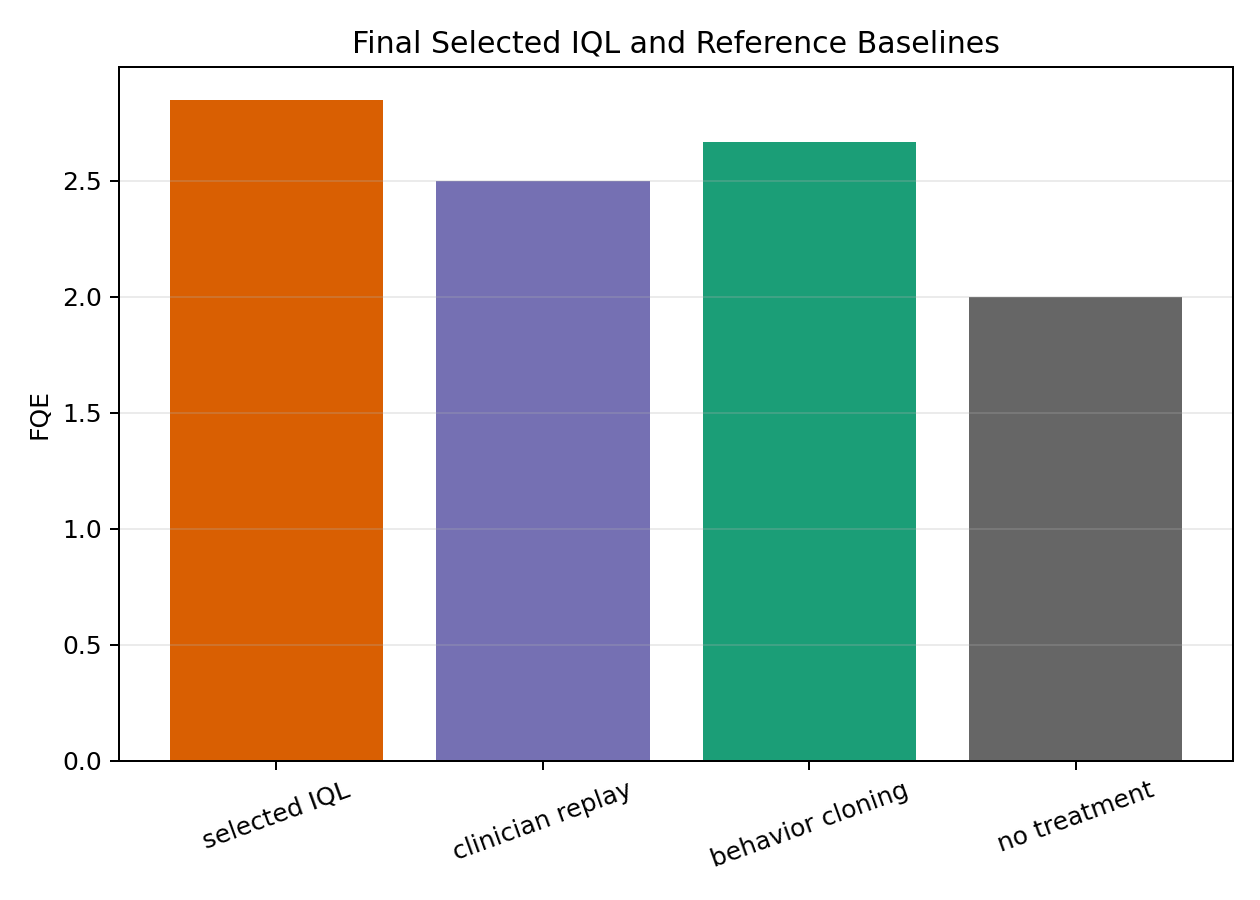
\includegraphics[width=.98\columnwidth]{figures/baseline_comparison.png}
  \caption{Final seçili IQL politikası ve referans baseline gösterimi. Seçili IQL değeri gerçek Aşama 2 değerlendirmesinden, referans baseline çubukları ise rapor artifactinde kullanılan karşılaştırma gösteriminden gelir.}
  \label{fig:baseline_comparison}
\end{figure}

\begin{figure}[t]
  \centering
  
\includegraphics[width=.98\columnwidth]{figures/seed_variance.png}
  \caption{Aşama 2 finalistleri için tekrarlı-tohum FQE değişkenliği. Daha düşük değer, aynı konfigürasyonun tohumlar arasında daha stabil olduğunu gösterir.}
  \label{fig:seed_variance}
\end{figure}

\section{Aksiyon ve Güvenlik Diagnostikleri}
Aksiyon dağılımı diagnostikleri zorunludur; çünkü öğrenilen klinik politika iyi value tahminleri üretirken observational veride nadir veya desteklenmeyen aksiyonlara kayabilir. Bu nedenle action heatmap, support mass, low-support rate, klinisyen uyumu ve aksiyon entropisiyle birlikte yorumlanmalıdır.

\begin{figure}[t]
  \centering
  
\includegraphics[width=.98\columnwidth]{figures/action_heatmap.png}
  \caption{Final politika analizi için üretilmiş aksiyon dağılımı heatmap'i. Tedavi gridi vazopresör ve sıvı şiddetinin ayrık kombinasyonlarını temsil eder.}
  \label{fig:action_heatmap}
\end{figure}

\begin{figure}[t]
  \centering
  
\includegraphics[width=.98\columnwidth]{figures/bootstrap_ci.png}
  \caption{Final seçili IQL politikasının üç tohum için hasta-düzeyi bootstrap WIS güven aralıkları. Güven aralıkları 50 bootstrap resample ile hesaplanmıştır ve düşük ESS nedeniyle temkinli yorumlanmalıdır.}
  \label{fig:bootstrap_ci}
\end{figure}

Klinik yorum için politika sürekli aşırı sıvı veya aşırı vazopresör öneriyor mu, `no treatment' aksiyonuna anormal şekilde collapse ediyor mu, düşük davranış desteği olan aksiyonları sık seçiyor mu, yüksek riskli alt gruplarda güvenlik uyarıları artıyor mu ve reward variant değişince politika dramatik şekilde değişiyor mu soruları kontrol edilmelidir. Protokolde ayrıca clinician action distribution, IQL policy action distribution, difference heatmap, low-support action rate, clinician agreement by subgroup, high-risk subgroup policy action frequency, training loss curves, validation metric curves, reward variant boxplot, LR regime comparison ve expectile/temperature comparison grafikleri raporlanabilir artifactler olarak tanımlanmıştır.

Aşama 2 finalistlerinde destek kütlesi yaklaşık 0.990--0.991, klinisyen exact-bin uyumu ise yaklaşık 0.401--0.418 aralığındadır. Kazanan politikanın tam-kutu uyumu 0.414 olduğu için kararların 0.586'lık kısmı klinisyen davranışıyla birebir aynı değildir; ancak desteklenmeyen aksiyon sapmasının 0.009 düzeyinde kalması, bu sapmaların büyük bölümünün veri desteği bulunan komşu tedavi yörüngeleri içinde gerçekleştiğini gösterir. Bu ayrım klinik olarak önemlidir: politika klinisyeni kopyalamaz, fakat davranış verisinin tamamen dışına da sıçramaz. Buna karşın ESS değerleri tüm finalistlerde 50 eşiğinin altındadır; bu nedenle WIS tabanlı sıralama yüksek varyans riskiyle birlikte raporlanmalıdır. ESS uyarısı saklansaydı rapor, gözlemsel veride yalnız az sayıda etkili trajectory ile desteklenen bir tahmini kesin sonuç gibi sunma riski taşırdı. Bu yüzden final karar ``klinik üstünlük'' değil, destek kısıtı belirtilmiş retrospektif OPE sonucu olarak ifade edilmiştir.

\section{Yeniden Üretilebilirlik ve Teknoloji Yığını}
Tamamlanan iş akışı, protokol incelemesinde belirlenen ana eksikleri karşılar: final IQL sweep runner, on sekiz konfigürasyonlu grid, workflow seviyesinde orkestrasyon, presweep audit, final-altı seçim mantığı, tekrarlı-tohum Aşama 2 birleştirmesi, baseline karşılaştırma artifactleri ve final grafik raporları. Üretilen artifact seti presweep audit sonucunu, Aşama 1 seçim tablosunu, Aşama 2 seed özetini, final metrics bundle'ı, baseline karşılaştırmasını ve beş grafik çıktısını içerir. Güncel Aşama 2 değerlendirmesi sonuçlarında on sekiz finalist-tohum satırı olarak saklanmıştır.

Teknoloji yığını Python ve `uv' tabanlı ortam yönetimi, yüksek hızlı `Polars' ve `PyArrow' tabanlı Parquet veri dönüşümü, `PyTorch' ve özelleştirilmiş `d3rlpy' tabanlı RL eğitimi, `Hydra' konfigürasyon yönetimi, `MLflow' deney takibi ve IEEE LaTeX raporlamasından oluşur. Device-agnostic tasarım sayesinde eğitim kodu MPS, CUDA veya otomatik cihaz seçimiyle çalışabilir. Bu altyapı ayrıştırılmasaydı deney sonuçları belirli bir donanıma veya elle değiştirilmiş konfigürasyonlara bağımlı hale gelirdi.

Her run için git commit hash, config dosyası, reward variant, LR regime, expectile, temperature, seed, dataset path, metadata path, split manifest seed, action bin artifact, training logs, checkpoint path, evaluation output ve figure paths kaydedilmelidir. Run isimlendirme şablonu reward, LR rejimi, IQL ayarı ve seed bilgisini birlikte taşıyan `iql\_reward\_lr\_setting\_seed' biçimindedir. Örneğin SOFA-shaped, actor-conservative, baseline ve seed 42 bilgileri aynı run adında saklanır. Bu sözleşme tutulmasaydı sonradan hangi checkpointin hangi veri ve konfigürasyonla üretildiği izlenemezdi.

\section{Sınırlar ve Etik Değerlendirme}
Bu çalışma retrospektif ve observational niteliktedir. Öğrenilen politika yatak başı tedavi önerisi olarak yorumlanmamalıdır. Durum temsili gizli klinik şiddeti, kontrendikasyonları, hekim niyetini ve ölçülmeyen confounding etkilerini tam olarak kapsayamaz. Gerçek klinik süreç POMDP niteliği taşır; eldeki state vektörü hekimin tüm yatak başı bilgisini içermez. Clinician action'ları observational olduğu için confounding içerir; örneğin daha hasta kişilere daha agresif vazopresör verilmesi, tedavinin zararlı görünmesine veya yanlış fayda atfedilmesine neden olabilir.

MIMIC-IV verisi PhysioNet credentialing, CITI training ve Data Use Agreement kapsamındaki yükümlülüklere tabidir; hasta verileri de-identified olsa da raporlama akademik ve etik sınırlar içinde kalmalıdır. FQE ve WIS prospektif klinik kanıt değildir; fonksiyon yaklaşımı, behavior policy tahmini, destek varsayımları ve variance profiline bağlıdır. ESS değerinin 50 eşiğinin altında kalması ve bootstrap resample sayısının sınırlı olması nedeniyle final politika sonucu klinik performans kanıtı olarak yorumlanmamalıdır.

\section{Gelecek Araştırma Yönleri}
Referans araştırma taslakları, bu çalışmanın güvenli IQL hattını daha ileri offline RL fikirleriyle genişletmek için üç somut yön göstermektedir. İlk yön, statik expectile yerine epistemic uncertainty ve yerel veri yoğunluğuna göre değişen dinamik expectile kalibrasyonudur. Yoğun destekli bölgelerde $\tau$ yükseltilerek daha agresif politika iyileştirme yapılabilir; seyrek ve belirsiz bölgelerde $\tau$ 0.5'e yaklaştırılarak davranış klonlamasına benzer güvenli güncelleme tercih edilebilir.

İkinci yön, sparse terminal mortalite sinyalini daha hızlı yaymak için adaptive multi-step trace blending kullanmaktır. Peng'in $Q(\lambda)$ fikri, yüksek güvenli trajectory bölümlerinde daha büyük $\lambda$, belirsiz veya düşük destekli geçişlerde daha küçük $\lambda$ kullanacak şekilde klinik veriye uyarlanabilir. Üçüncü yön, state-space manifold regularization için generative world-model veya diffusion tabanlı trajectory simülatörleridir. Böyle bir model, klinik olarak gerçekçi ama veri setinde seyrek görülen sınır durumları sentezleyerek value fonksiyonuna daha güvenli marjlar öğretebilir. Bu üç genişleme, mevcut raporun temel ilkesini korumalıdır: önce veri desteği ve leakage-free değerlendirme, sonra politika iyileştirmesi.

\section{Sonuç}
Geliştirilen IQL final tarama iş akışı, protokol düzeyindeki deney tasarımını sepsis tedavi politikası değerlendirmesi için yeniden üretilebilir bir offline pekiştirmeli öğrenme pipeline'ına dönüştürür. Rapor artık kohort seçiminden zaman penceresine, state/action/reward mühendisliğinden leakage-free preprocessing sözleşmelerine, IQL algoritma ayrıntılarından hiperparametre grid'ine, Aşama 1 finalist seçimi ve Aşama 2 çoklu-tohum değerlendirmesine kadar projenin bütün ana adımlarını içerir. Aşama 0 denetimi başarılıdır ve Aşama 1 altı çeşitli, destek-duyarlı finalist belirlemiştir. Güncel Aşama 2 sonucuna göre final konfigürasyon `iql\_sofa\_shaped\_conservative\_safe' olarak seçilmiştir. Bu model FQE=2.848, WIS=8.203 ve bootstrap WIS 95\% CI=4.963--10.817 ile final konfigürasyon olarak raporlanmıştır; ancak ESS=29.41 ile destek eşiğinin altındadır. Bu nedenle sonuç klinik değil metodolojik ve retrospektif OPE kanıtı olarak raporlanmalıdır.

\bibliographystyle{IEEEtran}
\bibliography{references}

\end{document}
